\hypertarget{RandomForest_8c}{
\section{Random\-Forest.c File Reference}
\label{RandomForest_8c}\index{RandomForest.c@{RandomForest.c}}
}
{\tt \#include \char`\"{}party.h\char`\"{}}\par


Include dependency graph for Random\-Forest.c:\begin{figure}[H]
\begin{center}
\leavevmode
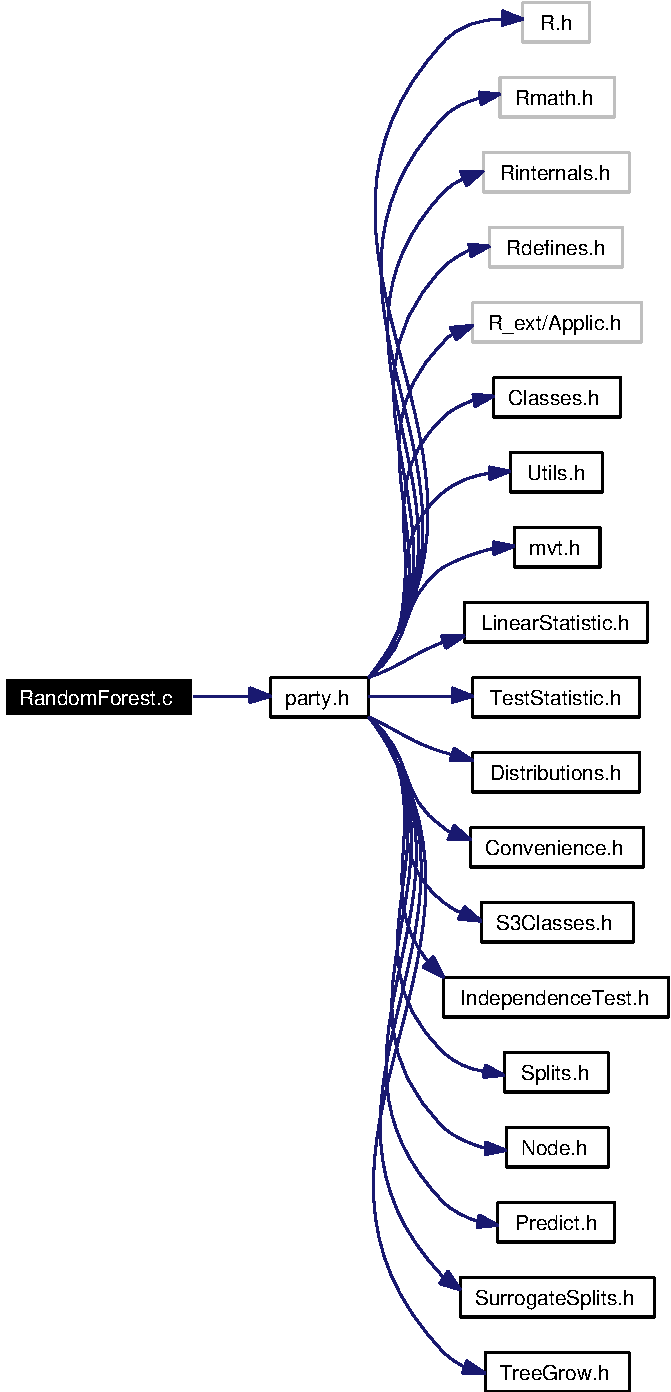
\includegraphics[width=178pt]{RandomForest_8c__incl}
\end{center}
\end{figure}
\subsection*{Functions}
\begin{CompactItemize}
\item 
void \hyperlink{RandomForest_8c_ccce6f00d55276c0a01b30651f1c206c}{C\_\-remove\_\-weights} (SEXP subtree)
\item 
SEXP \hyperlink{RandomForest_8c_4f54420cb561055a4e545f7e1359fb87}{R\_\-Ensemble} (SEXP learnsample, SEXP weights, SEXP bwhere, SEXP bweights, SEXP fitmem, SEXP controls)
\end{CompactItemize}


\subsection{Detailed Description}
Random forest with conditional inference trees

\begin{Desc}
\item[Author:]\begin{Desc}
\item[Author]hothorn \end{Desc}
\end{Desc}
\begin{Desc}
\item[Date:]\begin{Desc}
\item[Date]2007-07-23 10:02:09 +0200 (Mon, 23 Jul 2007) \end{Desc}
\end{Desc}


Definition in file \hyperlink{RandomForest_8c-source}{Random\-Forest.c}.

\subsection{Function Documentation}
\hypertarget{RandomForest_8c_ccce6f00d55276c0a01b30651f1c206c}{
\index{RandomForest.c@{Random\-Forest.c}!C_remove_weights@{C\_\-remove\_\-weights}}
\index{C_remove_weights@{C\_\-remove\_\-weights}!RandomForest.c@{Random\-Forest.c}}
\subsubsection[C\_\-remove\_\-weights]{\setlength{\rightskip}{0pt plus 5cm}void C\_\-remove\_\-weights (SEXP {\em subtree})}}
\label{RandomForest_8c_ccce6f00d55276c0a01b30651f1c206c}




Definition at line 11 of file Random\-Forest.c.

Referenced by C\_\-remove\_\-weights().\hypertarget{RandomForest_8c_4f54420cb561055a4e545f7e1359fb87}{
\index{RandomForest.c@{Random\-Forest.c}!R_Ensemble@{R\_\-Ensemble}}
\index{R_Ensemble@{R\_\-Ensemble}!RandomForest.c@{Random\-Forest.c}}
\subsubsection[R\_\-Ensemble]{\setlength{\rightskip}{0pt plus 5cm}SEXP R\_\-Ensemble (SEXP {\em learnsample}, SEXP {\em weights}, SEXP {\em bwhere}, SEXP {\em bweights}, SEXP {\em fitmem}, SEXP {\em controls})}}
\label{RandomForest_8c_4f54420cb561055a4e545f7e1359fb87}


An experimental implementation of random forest like algorithms \par
 \begin{Desc}
\item[Parameters:]
\begin{description}
\item[{\em learnsample}]an object of class `Learning\-Sample' \item[{\em weights}]a vector of case weights \item[{\em bwhere}]integer matrix (n x ntree) for terminal node numbers \item[{\em bweights}]double matrix (n x ntree) for bootstrap case weights \item[{\em fitmem}]an object of class `Tree\-Fit\-Memory' \item[{\em controls}]an object of class `Tree\-Control' \end{description}
\end{Desc}


Definition at line 33 of file Random\-Forest.c.

References get\_\-nobs(), and get\_\-ntree().

Here is the call graph for this function:\begin{figure}[H]
\begin{center}
\leavevmode
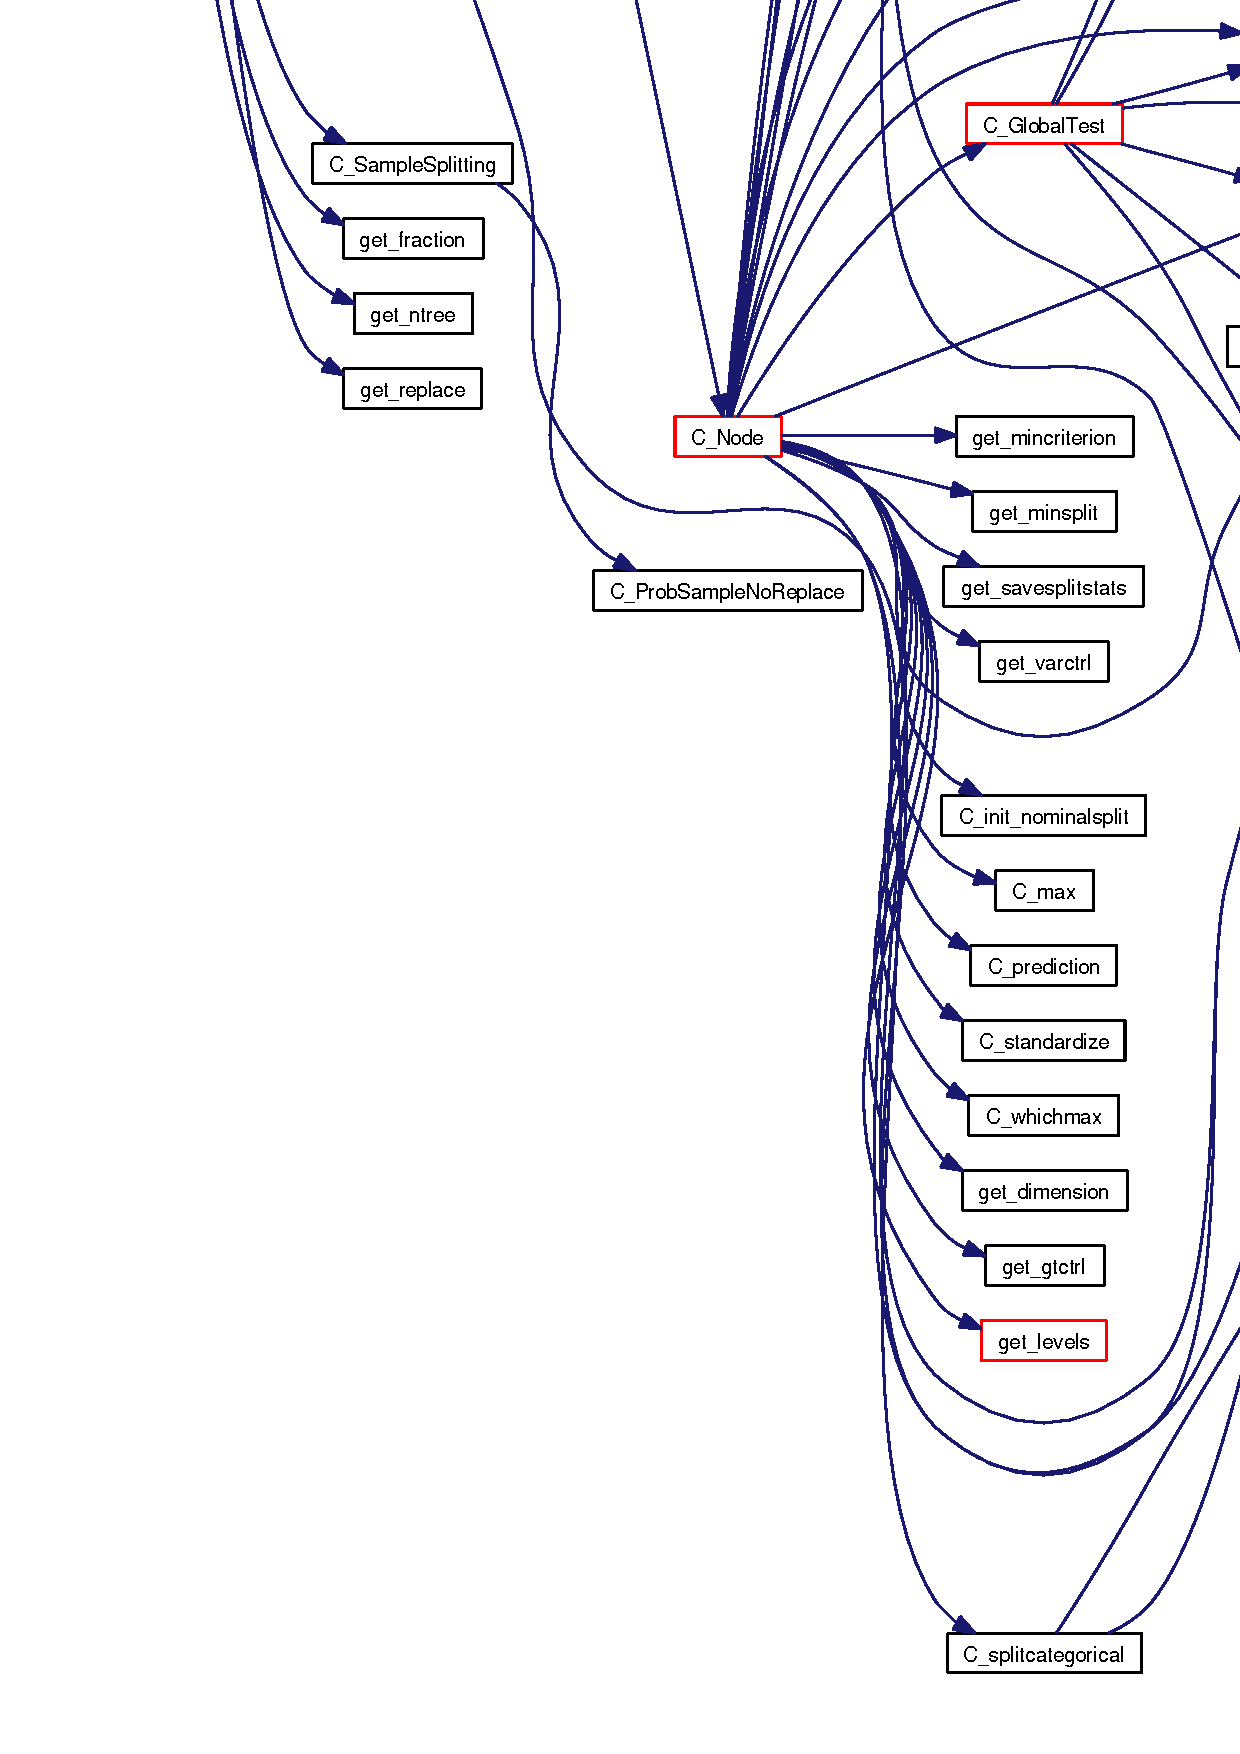
\includegraphics[width=103pt]{RandomForest_8c_4f54420cb561055a4e545f7e1359fb87_cgraph}
\end{center}
\end{figure}
